\PassOptionsToPackage{usenames}{color}
\documentclass[11pt,a4paper]{article}

\usepackage{relsize} % relative font sizes (e.g. \smaller). must precede ACL style
\usepackage{style/acl2015}
\usepackage[colorlinks=true,linkcolor=black,citecolor=black,filecolor=black,urlcolor=black]{hyperref}
\usepackage{natbib}

%\usepackage{times}
%\usepackage{latexsym}

\usepackage{microtype}
\usepackage{ dsfont }
\usepackage[boxed]{algorithm2e}
\renewcommand\AlCapFnt{\small}
\usepackage[small,bf,skip=5pt]{caption}
\usepackage{sidecap} % side captions
\usepackage{rotating}	% sideways
% \usepackage[pdftex]{graphicx}

% Italicize subparagraph headings
\usepackage{titlesec}
\titleformat*{\subparagraph}{\itshape}
\titlespacing{\subparagraph}{%
  1em}{%              left margin
  0pt}{% space before (vertical)
  1em}%               space after (horizontal)

% Numbered Examples and lists
\usepackage{lingmacros}
\newcommand{\exref}[1]{(\ref{#1})} % numbered example

\usepackage[shortlabels]{enumitem} % customizable lists
\setitemize{noitemsep,topsep=0em,leftmargin=*}
\setenumerate{noitemsep,leftmargin=0em,itemindent=13pt,topsep=0em}

\usepackage{xspace}
\usepackage{xparse} % for fancy custom macros (\NewDocumentEnvironment, etc.)

\newcommand{\indicator}[1]{I_{\{#1\}}} %{\mathds{1}_{\{#1\}}}


\usepackage{textcomp}
% \usepackage{arabtex} % must go after xparse, if xparse is used!
%\usepackage{utf8}
% \setcode{utf8} % use UTF-8 Arabic
% \newcommand{\Ar}[1]{\RL{\novocalize #1}} % Arabic text

\usepackage{framed}

\usepackage{listings}

\lstset{
  basicstyle=\itshape,
  xleftmargin=3em,
  aboveskip=0pt,
  belowskip=-3pt, %-.5\baselineskip, % correct for extra paragraph break inserted after listing
  literate={->}{$\rightarrow$}{2}
           {α}{$\alpha$}{1}
           {δ}{$\delta$}{1}
           {(}{$($}{1}
           {)}{$)$}{1}
           {[}{$[$}{1}
           {]}{$]$}{1}
           {|}{$|$}{1}
           {+}{\ensuremath{^+}}{1}
           {*}{\ensuremath{^*}}{1}
}

\usepackage{amssymb}	%amsfonts,eucal,amsbsy,amsthm,amsopn
\usepackage{amsmath}

\usepackage{mathptmx}	% txfonts
\usepackage[scaled=.8]{beramono}
\usepackage[scaled=.85]{helvet}
\usepackage[T1]{fontenc}
\usepackage[utf8x]{inputenc}

\usepackage{MnSymbol}	% must be after mathptmx

\usepackage{latexsym}


\addtolength{\textfloatsep}{-0.2cm}
\addtolength{\abovedisplayskip}{-0.2cm}
\addtolength{\belowdisplayskip}{-0.2cm}
%\addtolength{\abovecaptionskip}{-0.2cm}
%\addtolength{\belowcaptionskip}{-0.2cm}




% Tables
\usepackage{array}
\usepackage{multirow}
\usepackage{booktabs} % pretty tables
\usepackage{multicol}
\usepackage{footnote}
\newcolumntype{H}{>{\setbox0=\hbox\bgroup}c<{\egroup}@{}} % hidden column


\usepackage{url}
\usepackage[usenames]{color}
\usepackage{xcolor}

% colored frame box
\newcommand{\cfbox}[2]{%
    \colorlet{currentcolor}{.}%
    {\color{#1}%
    \fbox{\color{currentcolor}#2}}%
}

\usepackage[normalem]{ulem} % \uline
\usepackage{colortbl}
\usepackage{graphicx}
\usepackage{subcaption}
%\usepackage{tikz-dependency}
\usepackage{tikz}
%\usepackage{tree-dvips}
\usetikzlibrary{arrows,positioning,calc} 

\DeclareMathOperator*{\argmax}{arg\,max}
\DeclareMathOperator*{\argmin}{arg\,min}
%\setlength\titlebox{6.5cm}    % Expanding the titlebox


\usepackage{nameref}
\usepackage{cleveref}

% use \S for all references to all kinds of sections, and \P to paragraphs
% (sadly, we cannot use the simpler \crefname{} macro because it would insert a space after the symbol)
\crefformat{part}{\S#2#1#3}
\crefformat{chapter}{\S#2#1#3}
\crefformat{section}{\S#2#1#3}
\crefformat{subsection}{\S#2#1#3}
\crefformat{subsubsection}{\S#2#1#3}
\crefformat{paragraph}{\P#2#1#3}
\crefformat{subparagraph}{\P#2#1#3}
%\crefmultiformat{part}{\S#2#1#3}{ and~\S#2#1#3}{, \S#2#1#3}{, and~\S#2#1#3}
%\crefmultiformat{chapter}{\S#2#1#3}{ and~\S#2#1#3}{, \S#2#1#3}{, and~\S#2#1#3}
\crefmultiformat{section}{\S#2#1#3}{ and~\S#2#1#3}{, \S#2#1#3}{, and~\S#2#1#3}
\crefmultiformat{subsection}{\S#2#1#3}{ and~\S#2#1#3}{, \S#2#1#3}{, and~\S#2#1#3}
\crefmultiformat{subsubsection}{\S#2#1#3}{ and~\S#2#1#3}{, \S#2#1#3}{, and~\S#2#1#3}
\crefmultiformat{paragraph}{\P\P#2#1#3}{ and~#2#1#3}{, #2#1#3}{, and~#2#1#3}
\crefmultiformat{subparagraph}{\P\P#2#1#3}{ and~#2#1#3}{, #2#1#3}{, and~#2#1#3}
%\crefrangeformat{part}{\mbox{\S\S#3#1#4--#5#2#6}}
%\crefrangeformat{chapter}{\mbox{\S\S#3#1#4--#5#2#6}}
\crefrangeformat{section}{\mbox{\S\S#3#1#4--#5#2#6}}
\crefrangeformat{subsection}{\mbox{\S\S#3#1#4--#5#2#6}}
\crefrangeformat{subsubsection}{\mbox{\S\S#3#1#4--#5#2#6}}
\crefrangeformat{paragraph}{\mbox{\P\P#3#1#4--#5#2#6}}
\crefrangeformat{subparagraph}{\mbox{\P\P#3#1#4--#5#2#6}}
% for \label[appsec]{...}
\crefname{part}{Part}{Parts}
\Crefname{part}{Part}{Parts}
\crefname{chapter}{ch.}{ch.}
\Crefname{chapter}{Ch.}{Ch.}
\crefname{figure}{figure}{figures}
\crefname{appsec}{appendix}{appendices}
\Crefname{appsec}{Appendix}{Appendices}
\crefname{algocf}{algorithm}{algorithms}
\Crefname{algocf}{Algorithm}{Algorithms}
\crefname{enums,enumsi}{example}{examples}
\Crefname{enums,enumsi}{Example}{Examples}
\crefname{}{example}{examples} % lingmacros \toplabel has no internal name for the kind of label
\Crefname{}{Example}{Examples}
\crefformat{enums}{(#2#1#3)}
\crefformat{enumsi}{(#2#1#3)}
\crefformat{}{(#2#1#3)}
\crefrangeformat{enums}{\mbox{(#3#1#4--#5#2#6)}}
\crefrangeformat{enumsi}{\mbox{(#3#1#4--#5#2#6)}}

\ifx\creflastconjunction\undefined%
\newcommand{\creflastconjunction}{, and\nobreakspace} % Oxford comma for lists
\else%
\renewcommand{\creflastconjunction}{, and\nobreakspace} % Oxford comma for lists
\fi%

\newcommand*{\Fullref}[1]{\hyperref[{#1}]{\Cref*{#1}: \nameref*{#1}}}
\newcommand*{\fullref}[1]{\hyperref[{#1}]{\cref*{#1}: \nameref{#1}}}
\newcommand{\fnref}[1]{fn.~\ref{#1}} % don't use \cref{} due to bug in (now out-of-date) cleveref package w.r.t. footnotes
\newcommand{\Fnref}[1]{Fn.~\ref{#1}}


\newcommand{\backtick}[0]{\textasciigrave}


\NewDocumentEnvironment{itmize}{}{\begin{itemize}[noitemsep]}{\end{itemize}}
\NewDocumentEnvironment{enumrate}{}{\begin{enumerate}[noitemsep]}{\end{enumerate}}
\let\Item\item
\renewcommand\enddescription{\endlist\global\let\item\Item}
\NewDocumentEnvironment{describe}{}{\renewcommand\item[1][]{\Item \textbf{##1:} }\begin{itemize}}{\end{itemize}}
\NewDocumentEnvironment{edescribe}{}{\renewcommand\item[1][]{\Item \textbf{##1:} }\begin{enumerate}}{\end{enumerate}}

\newcommand{\exemplars}{\mathrm{ex}}
\newcommand{\fulltext}{\mathrm{ft}}

% Author comments
\usepackage{color}
\newcommand\bmmax{0} % magic to avoid 'too many math alphabets' error
\usepackage{bm}
\definecolor{orange}{rgb}{1,0.5,0}
\definecolor{mdgreen}{rgb}{0.05,0.6,0.05}
\definecolor{mdblue}{rgb}{0,0,0.7}
\definecolor{dkblue}{rgb}{0,0,0.5}
\definecolor{dkgray}{rgb}{0.3,0.3,0.3}
\definecolor{slate}{rgb}{0.25,0.25,0.4}
\definecolor{gray}{rgb}{0.5,0.5,0.5}
\definecolor{ltgray}{rgb}{0.7,0.7,0.7}
\definecolor{purple}{rgb}{0.7,0,1.0}
\definecolor{lavender}{rgb}{0.65,0.55,1.0}

% Settings for algorithm listings
% \lstset{
%   language=Python,
%   upquote=true,
%   showstringspaces=false,
%   formfeed=\newpage,
%   tabsize=1,
%   commentstyle=\itshape\color{lavender},
%   basicstyle=\small\smaller\ttfamily,
%   morekeywords={lambda},
%   emph={upward,downward,tc},
%   emphstyle=\underbar,
%   aboveskip=0cm,
%   belowskip=-.5cm
% }
%\renewcommand{\lstlistingname}{Algorithm}


\newcommand{\ensuretext}[1]{#1}
\newcommand{\cjdmarker}{\ensuretext{\textcolor{mdgreen}{\ensuremath{^{\textsc{CJ}}_{\textsc{D}}}}}}
\newcommand{\nssmarker}{\ensuretext{\textcolor{magenta}{\ensuremath{^{\textsc{NS}}_{\textsc{S}}}}}}
\newcommand{\mkmarker}{\ensuretext{\textcolor{red}{\ensuremath{^{\textsc{M}}_{\textsc{K}}}}}}
\newcommand{\stmarker}{\ensuretext{\textcolor{orange}{\ensuremath{^{\textsc{S}}_{\textsc{T}}}}}}
\newcommand{\nasmarker}{\ensuretext{\textcolor{blue}{\ensuremath{^{\textsc{NA}}_{\textsc{S}}}}}}
\newcommand{\jbmarker}{\ensuretext{\textcolor{orange}{\ensuremath{^{\textsc{J}}_{\textsc{B}}}}}}
\newcommand{\dbmarker}{\ensuretext{\textcolor{purple}{\ensuremath{^{\textsc{D}}_{\textsc{B}}}}}}
%\newcommand{\arkcomment}[3]{\ensuretext{\textcolor{#3}{[#1 #2]}}}
\newcommand{\arkcomment}[3]{}
\newcommand{\cjd}[1]{\arkcomment{\cjdmarker}{#1}{mdgreen}}
\newcommand{\nss}[1]{\arkcomment{\nssmarker}{#1}{magenta}}
\newcommand{\mk}[1]{\arkcomment{\mkmarker}{#1}{red}}
\newcommand{\st}[1]{\arkcomment{\stmarker}{#1}{orange}}
\newcommand{\jb}[1]{\arkcomment{\jbmarker}{#1}{blue}}
\newcommand{\db}[1]{\arkcomment{\dbmarker}{#1}{purple}}
\newcommand{\nascomment}[1]{\arkcomment{\nasmarker}{#1}{blue}}
\newcommand{\wts}{\mathbf{w}}
\newcommand{\g}{\mathbf{g}}
\newcommand{\f}{\mathbf{f}}
\newcommand{\x}{\mathbf{x}}
\newcommand{\y}{\mathbf{y}}
\newcommand{\overbar}[1]{\mkern 1.5mu\overline{\mkern-1.5mu#1\mkern-1.5mu}\mkern 1.5mu} % \bar is too narrow in math
\newcommand{\cost}{c}


\newcommand{\term}[1]{\textbf{#1}} % term being defined

\newcommand{\citeposs}[2][]{\citeauthor{#2}'s (\citeyear[#1]{#2})}
\newcommand{\Citeposs}[2][]{\Citeauthor{#2}'s (\citeyear[#1]{#2})}

% Space savers
% From http://www.eng.cam.ac.uk/help/tpl/textprocessing/squeeze.html
\addtolength{\textfloatsep}{-.3cm} % space between last top float or first bottom float and the text.
%\addtolength{\intextsep}{-1cm} % space left on top and bottom of an in-text float.
\addtolength{\abovedisplayskip}{-1cm} % space before maths
\addtolength{\belowdisplayskip}{-1cm} % space after maths
%\addtolength{\topsep}{-.5cm} %space between first item and preceding paragraph
%\setlength{\belowcaptionskip}{-.3cm}
\setlength{\intextsep}{0pt plus 2pt}   % default value 12pt plus 2pt minus 2pt


% customize \paragraph spacing
\makeatletter
\renewcommand{\paragraph}{%
  \@startsection{paragraph}{4}%
  {\z@}{.2ex \@plus 1ex \@minus .2ex}{-1em}%
  {\normalfont\normalsize\bfseries}%
}
\makeatother



% Special macros
\newcommand{\lbl}[1]{\textsc{#1}} % class label
\newcommand{\sst}[1]{\lbl{#1}} % supersense tag label
\newcommand{\nsst}[1]{\sst{n:#1}} % noun supersense tag label
\newcommand{\vsst}[1]{\sst{v:#1}} % verb supersense tag label


\newcommand{\tg}[1]{\texttt{#1}}	% supersense tag name
\newcommand{\gfl}[1]{%\renewcommand\texttildelow{{\lower.74ex\hbox{\texttt{\char`\~}}}} % http://latex.knobs-dials.com/
\mbox{\textsmaller{\texttt{#1}}}}	% supersense tag symbol
 \newcommand{\tagdef}[1]{#1\hfill} % tag definition
\newcommand{\tagt}[2]{\ensuremath{\underset{\textrm{\textlarger{\tg{#2}}}\strut}{\w{#1}\rule[-.3\baselineskip]{0pt}{0pt}}}} % tag text (a word or phrase) with an SST. (second arg is the tag)
\newcommand{\glosst}[2]{\ensuremath{\underset{\textrm{#2}}{\textrm{#1}}}} % gloss text (a word or phrase) (second arg is the gloss)
\newcommand{\AnnA}[0]{\mbox{\textbf{Ann-A}}} % annotator A
\newcommand{\AnnB}[0]{\mbox{\textbf{Ann-B}}} % annotator B
\newcommand{\sys}[1]{\mbox{\textbf{#1}}}   % name of a system (one of our experimental conditions)
\newcommand{\dataset}[1]{\mbox{\textsc{#1}}}	% one of the datasets in our experiments
\newcommand{\datasplit}[1]{\mbox{\textbf{#1}}}	% portion one of the datasets in our experiments

\newcommand{\fnf}[1]{\textsc{\textsf{#1}}} % FrameNet frame
\newcommand{\fnr}[1]{\textbf{\textsf{#1}}} % FrameNet role (frame element name)
\newcommand{\fnlu}[1]{\textsf{#1}} % FrameNet lexical unit (predicate)
\newcommand{\pbf}[1]{\mbox{\textsf{#1}}} % PropBank frame (roleset)
\newcommand{\pbr}[1]{\textbf{\textsf{#1}}} % PropBank role (numbered or modifier argument label)
\newcommand{\vpred}[1]{\textbf{#1}} % verb predicate


%\newcommand{\lex}[1]{\textsmaller{\textsf{\textcolor{slate}{\textbf{#1}}}}}	% example lexical item
\newcommand{\lex}[1]{\textit{#1}} % lexical item/lexical example
\newcommand{\pex}[1]{\textit{#1}} % phrasal example - don't index by default

%\newcommand{\w}[1]{\textit{#1}}	% word
\newcommand{\gap}[0]{\ \ } % space around gap contents
\newcommand{\tat}[0]{\textasciitilde}

\newcommand{\shortlong}[2]{#1} % short vs. long version of the paper
\newcommand{\confversion}[1]{#1}
\newcommand{\srsversion}[1]{}
\newcommand{\finalversion}[1]{}
%\newcommand{\finalversion}[1]{}
\newcommand{\shortversion}[1]{#1}
\newcommand{\considercutting}[1]{#1}
\newcommand{\longversion}[1]{} % ...if only there were more space...
\newcommand{\subversion}[1]{#1} % for the submission version only
\newcommand{\draftnotice}[1]{} % for the draft version only
%\newcommand{\subversion}[1]{}

%%%%%%%%%% HYPHENATION

\hyphenation{WordNet}
\hyphenation{WordNets}
\hyphenation{FrameNet}
\hyphenation{SemCor}
\hyphenation{SemEval}
\hyphenation{ParsedSemCor}
\hyphenation{VerbNet}
\hyphenation{PennConverter}
\hyphenation{an-aly-sis}
\hyphenation{an-aly-ses}
\hyphenation{base-line}
\hyphenation{comb-over}
\hyphenation{de-ve-lop-ed}
\hyphenation{news-text}
\hyphenation{nomi-nal}
\hyphenation{per-cept}
\hyphenation{per-cepts}
\hyphenation{post-edit-ing}
\hyphenation{shriv-eled}
\hyphenation{Huddle-ston}

\title{Frame-Semantic Role Labeling with Heterogeneous Annotations}

% Nathan Schneider, Shay B. Cohen, and Noah A. Smith 
% \author{Nathan Schneider \quad Emily Danchik \quad Chris Dyer \quad Noah A. Smith \\
% 	    School of Computer Science\\
% 	    Carnegie Mellon University\\
% 	    Pittsburgh, PA 15213, USA\\
% 	    {\tt \{nschneid,emilydan,cdyer,nasmith\}@cs.cmu.edu}}

% \author{Author 1\\
% 	    XYZ Company\\
% 	    111 Anywhere Street\\
% 	    Mytown, NY 10000, USA\\
% 	    {\tt author1@xyz.org}
% 	  \And
% 	Author 2\\
%   	ABC University\\
%   	900 Main Street\\
%   	Ourcity, PQ, Canada A1A 1T2\\
%   {\tt author2@abc.ca}}

%\date{}

\begin{document}
\maketitle
\begin{abstract}
We consider the task of identifying and labeling the semantic
arguments of a predicate that evokes a FrameNet frame.  This task is
challenging because there are only a few thousand fully annotated
sentences for supervised training.  Our approach augments an existing %, state-of-the-art\nss{SEMAFOR is no longer SOTA!}
model with features derived from FrameNet and PropBank and with
partially annotated exemplars from FrameNet.  We observe a 4\% absolute increase in $F_1$ 
%\mk{why percentage for $F_1$? i dont think it is the norm}\nss{yes, it is typical in NLP}
versus the original model.

% The high cost of semantic structure annotation is a major obstacle 
% to automating semantic analysis with broad coverage.
% %The fully annotated datasets that exist are often small, 
% %hindering the accuracy and domain robustness of models trained on them.
% %However, 
% %
% % Low-resource tasks may benefit from exploiting \emph{out-of-domain} annotated data, 
% % as well as data with \emph{different} (but related) forms of annotation,
% % for additional training data or features.
% This paper considers the argument identification and classification subtask 
% of frame-semantic parsing.
% % To date, systems evaluated on the full-sentence FrameNet parsing task 
% % have relied exclusively upon a small corpus of full-text annotations 
% % for learning to recognize arguments. 
% We augment supervised learning with additional 
% ``indirect'' training data and features 
% so as to leverage resources internal and external to FrameNet (e.g., PropBank). 
% Experiments demonstrate that these resources are valuable for 
% more accurate and robust frame-semantic role labeling,
% with the best model achieving nearly a 4-point increase in $F_1$ over the
% \st{SOTA?} baseline.
\end{abstract}

\section{Introduction}

Paucity of data resources is a challenge for semantic analyses like
frame-semantic parsing \citep{gildea-02,das-14} using the
FrameNet lexicon \citep{baker-98}.\footnote{\url{http://framenet.icsi.berkeley.edu}}
Given a sentence, a frame-semantic parse maps word tokens
to \textbf{frames} they evoke, and for each frame, finds and labels
its \textbf{argument} phrases  
with frame-specific \textbf{roles}. 
An example appears in \cref{fig:harbor-fn}. %; it will be explained in detail in \cref{sec:fn}.

In this paper, we address this \textbf{argument identification} 
subtask, a form of semantic role labeling (SRL), 
a task introduced by \citet{gildea-02} using an earlier version of FrameNet.
Our contribution addresses the paucity of annotated data for training 
using  standard domain
adaptation techniques.  We exploit three annotation sources:
\begin{itemize}
  \item the frame-to-frame relations in FrameNet, by using
  hierarchical features to share statistical strength among related roles
  (\cref{sec:hierfeats}),
  \item FrameNet's corpus of partially-annotated \textbf{exemplar} sentences,
  by using ``frustratingly easy'' domain adaptation (\cref{sec:frust}), and
  \item a PropBank-style SRL system, by using guide features (\cref{sec:guide}).
\end{itemize}
% We show that these internal and external resources improve frame-semantic
% parsing, as evaluated on full-text text annotations.
These expansions of the \emph{training corpus} and the \emph{feature set}
for supervised argument identification  are integrated into SEMAFOR
\citep{das-14},  the leading open-source frame-semantic parser for English.\footnote{\url{http://www.ark.cs.cmu.edu/SEMAFOR}} 
We observe a 4\% $F_1$ improvement in argument identification on the
FrameNet test set, leading to a 1\% $F_1$ improvement on the full
frame-semantic parsing task \nascomment{this point was not explained
  in experiments; either cut it or make sure there's a follow up}.

\begin{figure}
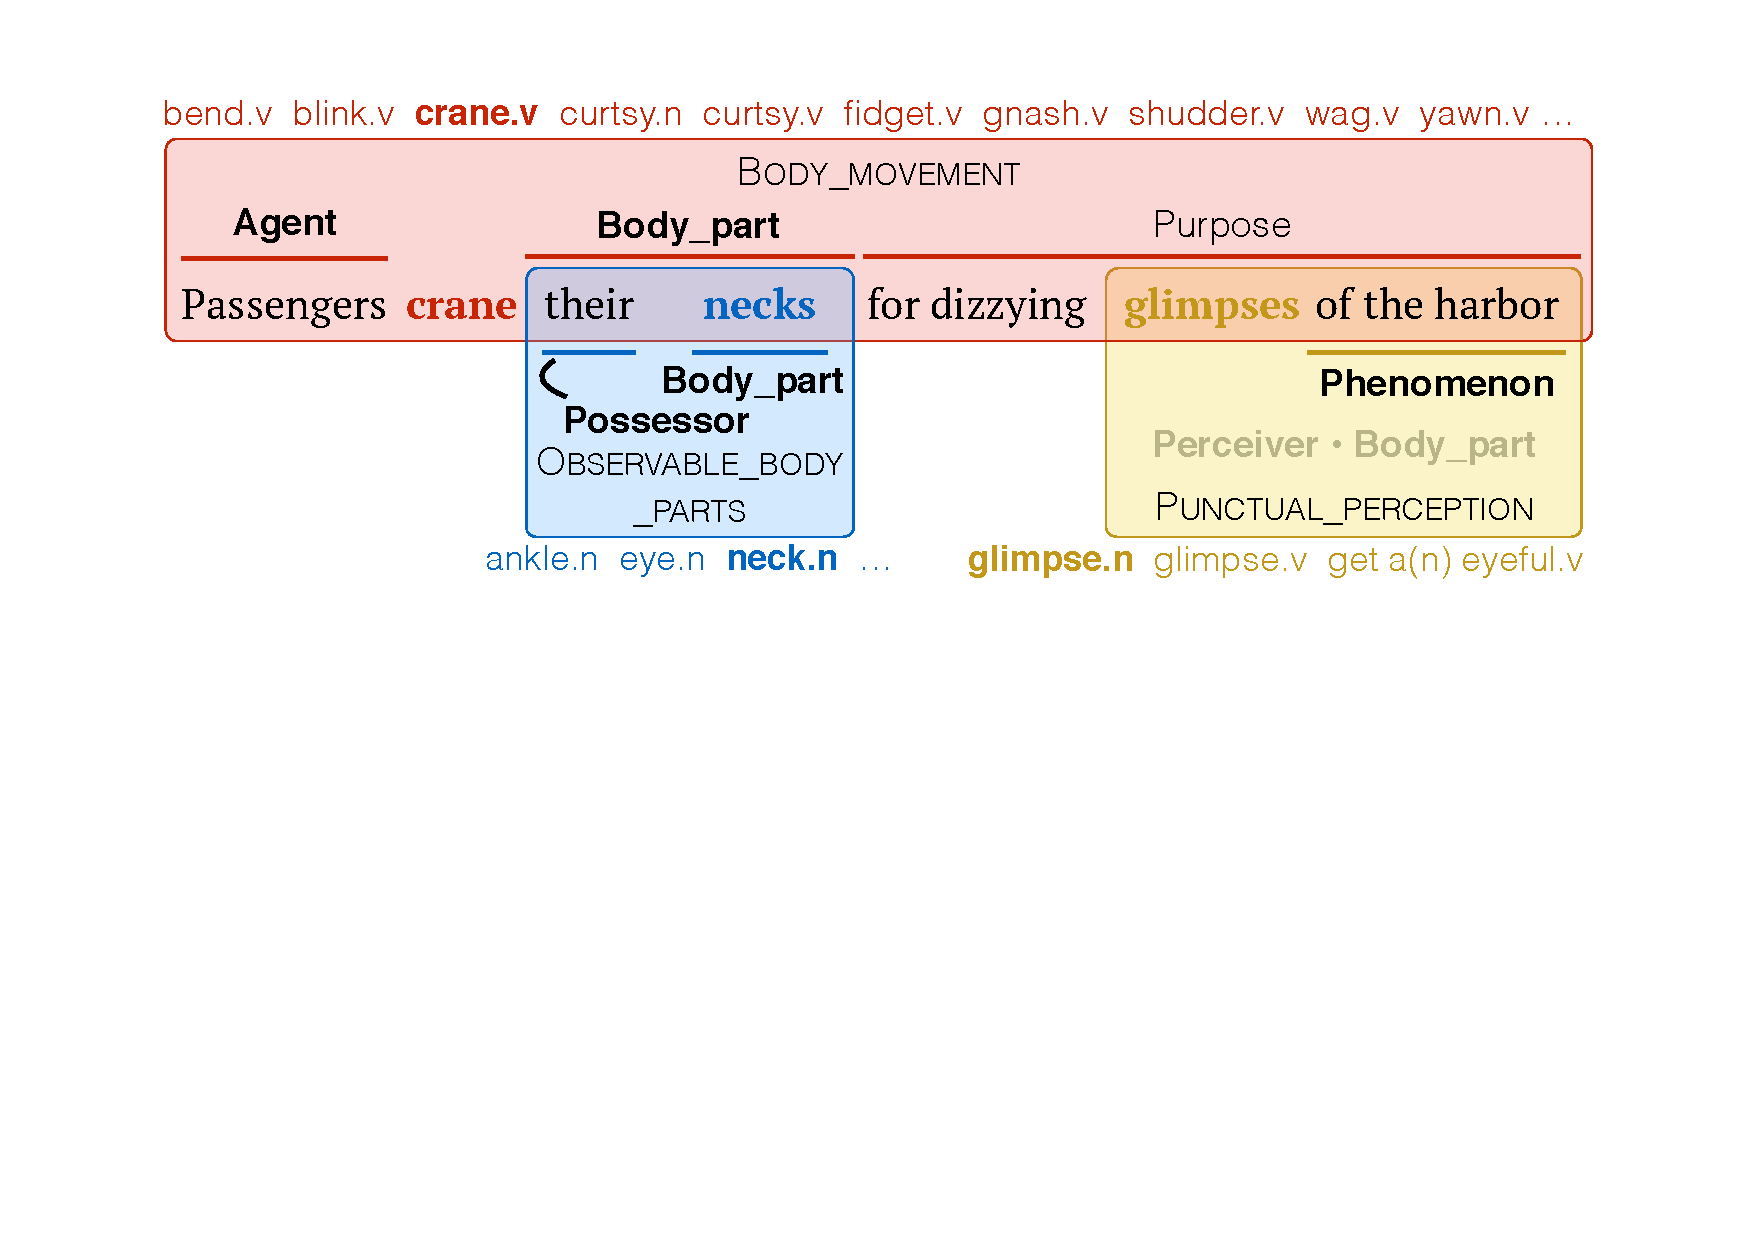
\includegraphics[width=\columnwidth]{fig/harbor-fn.pdf}
\caption{Example sentence from FrameNet full-text annotation. 
3~frames and their arguments are shown: 
\fnf{Body\_movement} is evoked by \textit{crane},
\fnf{Observable\_body\_parts} by \textit{necks}, 
and \fnf{Punctual\_perception} by \textit{glimpse}.
(Further, \textit{harbor} is annotated as evoking the \fnf{Locale\_by\_use} frame 
and doubles as its sole argument; not shown.) 
Horizontal lines representing argument spans 
are labeled with role names.}
\label{fig:harbor-fn}
\end{figure}

%\begin{figure}
%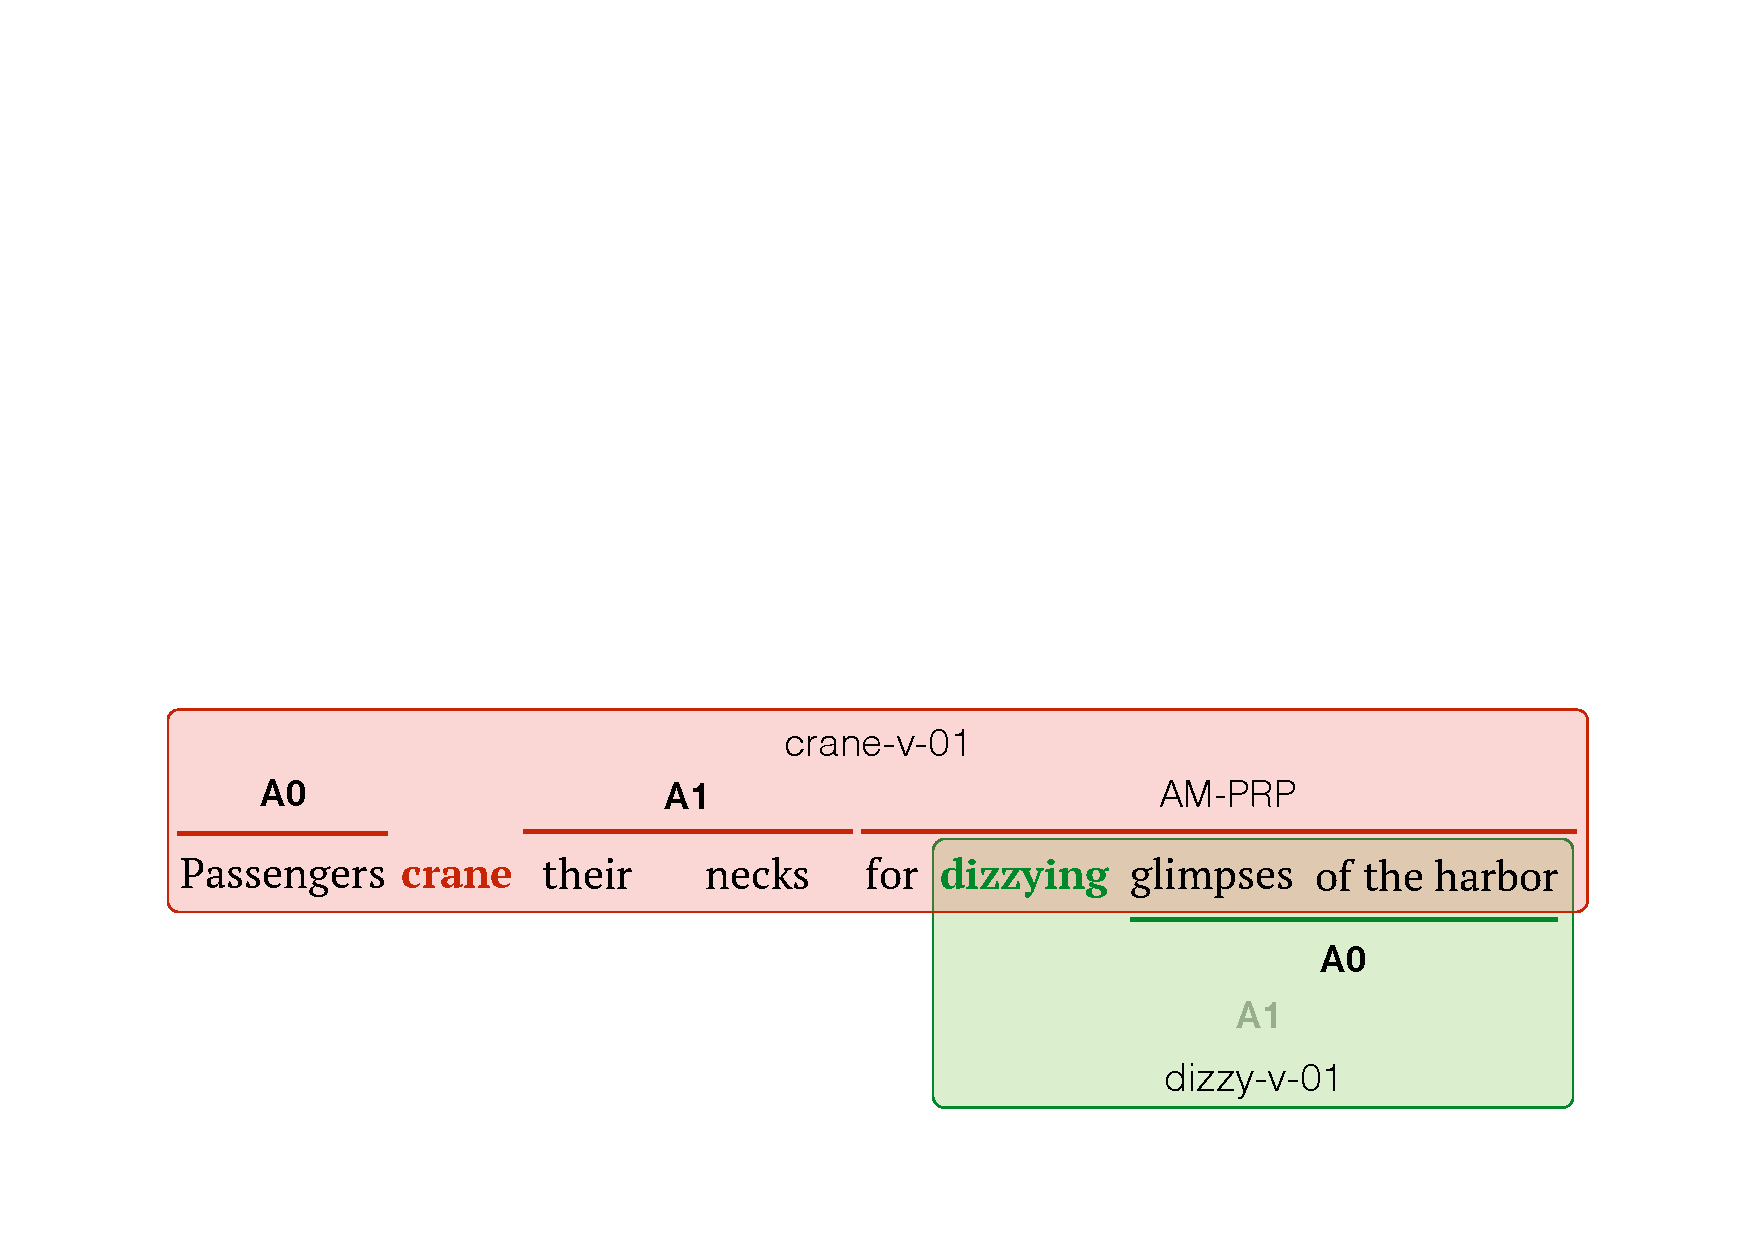
\includegraphics[width=\columnwidth]{fig/harbor-pb.pdf}
%\caption{Ideal PropBank (\cref{sec:pb}) annotations for verbs. Though PB uses lexical frames rather than deep frames,
%there are clear similarities to the FrameNet annotations in \cref{fig:harbor-fn}.}
%\label{fig:harbor-pb}
%\end{figure}





% \section{Data}\label{sec:data}

\section{FrameNet}\label{sec:fn}

%\nss{incl. data analysis of differences from full-text}

%\nss{w/in each mention: genre/overall vocabulary; coverage and distributions of predicates, FE labels; oracle coverage of FT test}

% \subsection{FrameNet}\label{sec:fn}

FrameNet represents events, scenarios, and relationships 
with an inventory of \textbf{frames} (such as \fnf{Shopping}, \fnf{Scarcity}, and \fnf{Shoot\_projectiles}). 
Each frame is associated with a set of \textbf{roles} (or \textbf{frame elements}) 
called to mind in order to understand the scenario,
and lexical \textbf{predicates} (verbs, nouns, adjectives, and adverbs) capable of 
evoking the scenario. 
For example, the \fnf{Body\_movement} frame has \fnr{Agent} and \fnr{Body\_part} as its core roles, 
and lexical entries including verbs such as \fnlu{bend}, \fnlu{blink}, \fnlu{crane}, and \fnlu{curtsy}, 
plus the noun use of \fnlu{curtsy}.
%the frame description states,
%``This frame contains words for motions or actions an \fnr{Agent} performs using some part of his/her body.''
\finalversion{
In the annotated sentence in \cref{fig:harbor-fn},
\fnf{Body\_movement} is evoked by \textit{crane}, and 3~of its roles are filled by overt arguments: 
the 2~core roles (\fnr{Agent}, \fnr{Body\_part}) happen to be filled by noun phrases 
(\textit{passengers}, \textit{their necks}), while the non-core role \fnr{Purpose} is filled by a 
prepositional phrase adjunct (\textit{for dizzying glimpses of the harbor}).
}
In FrameNet~1.5, there are over 1,000 frames and 12,000~lexical predicates.

%\nss{mention somewhere?: roles may be implicit, but are often realized in the sentence.}


\subsection{Hierarchy}

The FrameNet lexicon is organized as a network, with several kinds of \textbf{frame-to-frame relations} 
linking pairs of frames and (subsets of) their arguments \citep{ruppenhofer-10}. 
In this work, we consider two kinds of frame-to-frame relations:
\paragraph{Inheritance:} 
E.g., \fnf{Robbery} inherits from \fnf{Committing\_crime}, which inherits from \fnf{Misdeed}. 
Crucially, roles in inheriting frames are mapped to corresponding roles in inherited frames: \fnf{Robbery}.\fnr{Perpetrator} links to
\fnf{Committing\_crime}.\fnr{Perpetrator}, which links to \fnf{Misdeed}.\fnr{Wrongdoer}, and so forth.

%E.g., \fnf{Punctual\_perception} (e.g., \fnlu{glimpse.v}) inherits from 
%\fnf{Perception\_experience} (e.g., \fnlu{see.v}), which inherits from \fnf{Perception}. 
%Other frames inheriting from \fnf{Perception} include \fnf{Sensation} (e.g., \fnlu{sight.n}) and  
%\fnf{Becoming\_aware} (e.g., \fnlu{notice.v}). 
%Crucially, roles in inheriting (conceptually more specific) frames are mapped 
%where they correspond to a role in the inherited frame: so \fnf{Punctual\_perception}.\fnr{Perceiver} links to \fnf{Perception\_experience}.\fnr{Perceiver\_passive}, 
%which links to \fnf{Perception}.\fnr{Perceiver}, and so forth.
%, which links to \fnf{Sensation}.\fnr{Perceiver\_passive} and \fnf{Becoming\_aware}.\fnr{Cognizer}.

\paragraph{Subframe:} This indicates a subevent within a complex event. 
E.g., the \fnf{Criminal\_process} frame groups together subframes 
\fnf{Arrest}, \fnf{Arraignment} and \fnf{Trial}.
%\fnf{Arrest}, \fnf{Arraignment}, \fnf{Trial}, and \fnf{Sentencing}. 
\fnf{Criminal\_process}.\fnr{Defendant}, for instance, is mapped to 
\fnf{Arrest}.\fnr{Suspect}% \fnf{Arraignment}.\fnr{Defendant}, 
\finalversion{
\fnf{Trial}.\fnr{Defendant}, and \fnf{Sentencing}.\fnr{Convict}
}.
%Other salient participants in the complex event %(such as the crime for which someone is arrested, tried, etc.)\ 
%are similarly mapped via Subframe relations.
% This permits an inference that a person tried for a crime likely
% has been or will be arrested, arraigned, and sentenced for that crime.

We say that a $\textit{parent}$ of a
role is one that has either the \textbf{Inheritance} or \textbf{Subframe}
relation to it.\nss{clarify?}
There are 4,138 \textbf{Inheritance} and 589 \textbf{Subframe} links among role
types in FrameNet 1.5.

Prior work has %noted that the preponderance of role labels in FrameNet poses a challenge, and have
considered various ways of grouping role labels together in order to share statistical strength. 
\citet{matsubayashi-09} observed small gains from using the \textbf{Inheritance} relationships (like we do here), 
and also from grouping by the role name (SEMAFOR already incorporates such features).
% Their evaluation was on a simpler subtask of argument classification, and our experiments confirm that their results hold for argument identification as well as classification.
\citet{baldewein-04} learn latent clusters of roles and role-fillers, reporting mixed results.
Our approach is described in \cref{sec:hierfeats}.

\subsection{Annotations}
Statistics for the annotations appear in \cref{tbl:datastats}.\\
\textbf{Full-text (FT):} This portion of the FrameNet corpus consists of documents and has about 5,000
sentences for which annotators assigned frames and arguments to as many words as possible.
Beginning with the SemEval-2007 shared task on FrameNet analysis,
frame-semantic parsers have been trained and evaluated on the full-text data
% of the FrameNet corpus
 \citep{baker-07,das-14}.\footnote{Though these 
were \emph{annotated} at the document level, and train/dev/test splits are by document, the frame-semantic parsing 
is currently restricted to the sentence level.}
% Beginning with the SemEval-2007 shared task on FrameNet analysis \citep{baker-07},
% frame-semantic parsers have been trained and evaluated on the \textbf{full-text (FT)}\footnote{Though these 
% were \emph{annotated} at the document level, and train/dev/test splits are by document, the frame-semantic parsing 
% is currently restricted to the sentence level.} portion 
% of the FrameNet corpus. %This consists of documents for which annotators made an effort to assign frames and arguments to as many words as possible. 
% 
% \finalversion{The frame defines 19~additional non-core roles, none of which have an argument in the example.
% In frame semantics, non-core roles are considered to be \emph{conceptually} optional; 
% core roles may or may not be \emph{syntactically} optional, but if not locally specified they are 
% expected to be available from context, or else implicit.
% For example, \fnf{Punctual\_perception}---evoked in this case by \textit{glimpses}---is annotated 
% as missing 2~of its core roles. A human listener would resolve the identity of the \fnr{Perceiver} 
% from the wider context and the \fnr{Body\_part} from world knowledge. }
% 
% \finalversion{In some cases, FT annotation involved creating a new frame or adding a new lexical unit to an existing frame. 
% In other cases, words that in principle should be considered to evoke a frame were left unannotated 
% because they did not match any existing lexical units. 
% This was the case for \textit{passengers} and \textit{dizzying} in \cref{fig:harbor-fn}.}
The full-text documents represent a mix of genres, prominently including travel guides 
and bureaucratic reports about weapons stockpiles. 
%FrameNet~1.5 has about 5,000 full-text sentences in total. 
% , and an example annotated sentence in \cref{fig:harbor-fn}.

%\nss{Annotation density: (proportion of tokens evoking a frame. breakdown by POS?)}

\begin{table}\centering\small
\begin{tabular}{@{}p{2.25cm}r@{~~}r@{~~}r@{~~}r@{}}
%\toprule
\normalfont & \multicolumn{2}{c}{\textbf{\hspace{40pt}Full-Text}} & \multicolumn{2}{c}{\textbf{Exemplars}} \\
& \multicolumn{1}{c}{\hspace{30pt}\textit{train}} & \multicolumn{1}{c}{\textit{test}} & \multicolumn{1}{c}{\textit{train}} & \multicolumn{1}{c}{\textit{test}} \\
\midrule
Sentences  & 2,780 & 2,420 & 137,515 & 4,132 \\
Frames & 15,019 & 4,458 & 137,515 & 4,132 \\
Overt arguments & 25,918 & 7,210 & 278,985 & 8,417 \\
\midrule
\multicolumn{5}{c}{\textsc{types}} \\
Roles & 2,644 & 1,420 & 4,821 & 1,224 \\
\multicolumn{2}{@{}l}{Unseen frames  \quad \textit{vs.~train:}} & 46 & & 0 \\
\multicolumn{2}{@{}l}{Roles in unseen frames \quad \textit{vs.~train:}} & 178 & & 0 \\
\multicolumn{2}{@{}l}{Unseen roles \quad \textit{vs.~train:}} & 289 & & 38 \\
\multicolumn{2}{@{}l}{Unseen roles \quad \textit{vs.~combined train:}} & 103 & & 32 \\
\end{tabular}
\caption{Characteristics of the training and test data. (These statistics exclude the development set, which contains 4,463 frames over 746 sentences.)
\nss{above role types, add frame types?}}
\label{tbl:datastats}
\end{table}


%\subsection{Exemplars}\label{sec:exemplars}

%\st{TODO: shorten exemplar section}
%\mk{$\uparrow$ Done I guess}
%Conceived primarily as a lexicography project, 
%However, most FrameNet annotations serve to illustrate the argument structure potential 
%of particular predicates. 
% When predicates are added to a frame, 
% a large set of source corpora (primarily, the British National Corpus) covering a wide range of genres
% is searched for various syntactic patterns, 
% and a lexicographer identifies a selection, or \textbf{subcorpus}, of sentences 
% illustrating the predicate's behavior \citep{boas-05}.
% The subcorpus sentences are then annotated, but \emph{only with respect to the predicate in question}.
\noindent\textbf{Exemplars:} To document a given predicate, lexicographers manually select corpus examples and annotate them
\emph{only with respect to the predicate in question}.
These singly-annotated sentences from FrameNet are called lexicographic \textbf{exemplars}.
%The subset of exemplars containing argument annotations is described in \cref{tbl:datastats}.
There are over 140,000 sentences containing argument annotations % (an additional 35,000 exemplar sentences contain no overt arguments).
and relative to the FT dataset, these contain an order of magnitude more frame annotations
and over two orders of magnitude 
more sentences. As these were manually selected, the rate of overt arguments per frame
is noticeably higher than in the FT data.
% Because we are conditioning on the identified frame, 
% the fact that the exemplar dataset has just one annotated frame per sentence
% is not a concern in argument identification. However, the 
%But because exemplars have been manually selected, the rate of overt arguments per frame 
%is noticeably higher than in the full-text data, which potentially biases the 
%predictions of models trained on exemplars.\nss{cite \citep{palmer-10-eval} somewhere, maybe here}
%model's tendency to predict certain kinds of arguments in a way that is not statistically representative of a natural corpus.
The exemplars formed the basis of early studies of frame-semantic role
labeling \citep[e.g.,][]{gildea-02,thompson-03,fleischman-03,litkowski-04,kwon-04}.
Exemplars have not yet been exploited successfully to improve
role labeling performance on the more realistic FT task.\footnote{\citet{das-11,das-12} investigated semi-supervised techniques using the exemplars and WordNet for frame identification.
\citet{hermann-14} also improve frame identification by mapping frames
and predicates into the same continuous vector space, allowing
statistical sharing.}
% In this work, we seek to leverage these exemplar sentences. 
% We deem it worthwhile to %(a)~
% investigate whether the exemplars 
% can be used to improve performance on the full-text evaluation, 
% compensating for the scarcity of full-text training data.%,
% and (b)~to evaluate SRL performance on a held-out set of exemplars, 
% given that these exemplars represent a much broader range of genres, frames, and predicates 
% than the full-text data.\nss{TODO: quantify number of additional frames and predicates relative to FT-test!}
% This second evaluation, we believe, will give a useful indication of the robustness of the SRL model.

% as well as the (type-level) hierarchical structure of the FrameNet lexicon. 

% Each frame in the Berkeley FrameNet lexicon is intended to represent a gestalt scene.
% The frame definition includes: a descriptive name;
% a set of \textbf{core roles} representing participants and props that are crucial
% to understanding the scene; a set of \textbf{non-core roles} such as circumstantial
% information (time, place, manner, purpose, etc.);
% an English textual description of the scene and how its roles relate to one another;
% and a set of English predicates that can evoke the scene.

\finalversion{
\subsection{PropBank}\label{sec:pb}
\st{TODO: shorten PB section. we should spend less time talking about PB, and
more time talking about the specific SRL system we use.}
PropBank \citep[PB;][]{palmer-05} is a lexicon and corpus of predicate--argument
structures that takes a shallower approach than FrameNet. Whereas FrameNet frames cluster lexical predicates that evoke similar kinds of scenarios (with the same kinds of roles), 
and these frames are organized in a network, 
PropBank frames are purely lexical and there are no formal relations between different predicates 
or their roles. Further, PropBank's sense distinctions are generally coarser-grained than FrameNet's.
An example PB-annotated sentence is shown in \cref{fig:harbor-pb}.
}
\finalversion{PropBank does represent lexical ambiguity---e.g., the verb \textit{order} is ambiguous 
in PropBank between \pbf{order-v-01} ``impelled action'' and \pbf{order-v-02} ``request to be delivered''---but
PropBank's sense distinctions are generally coarser-grained than FrameNet's.}

\finalversion{
%Within sense-disambiguated PropBank frames, or \textbf{rolesets}, 
Core roles are defined with textual descriptions and assigned numbers. 
E.g., \pbf{order-v-02} defines: \pbr{A0} ``orderer'', 
\pbr{A1} ``thing ordered'', \pbr{A2} ``benefactive, ordered-for'', 
and \pbr{A3} ``source''.
Following \citeposs{dowty-91} theory of proto-roles, PropBank rolesets use \pbr{A0} for proto-agents 
and \pbr{A1} for proto-patients, but in general, there is much less consistency 
in interpretation of core roles across lexical predicates for PropBank than there is for FrameNet.
Another difference is that PropBank's non-core roles---named \pbr{AM-*}, 
such as \pbr{AM-PRP} for purposes---are not frame-specific.\footnote{\Citet{ellsworth-04} 
has a more extensive discussion of differences between PropBank's and FrameNet's conventions.}
Despite these differences, there is often a great deal in common between 
FrameNet-style and PropBank-style analyses, as should be apparent from comparing 
\cref{fig:harbor-fn} and \cref{fig:harbor-pb}.
}

\finalversion{
PropBank provides one million words of fully annotated English sentences.
% The major benefit to PropBank is that it includes a large and comprehensively
% annotated corpus.
% We hypothesize that leveraging this large corpus indirectly 
% can reap rewards for FrameNet-style SRL. 
% We use PropBank analyses as a signal in the FrameNet
% argument identification task 
% by preprocessing
% sentences with a PropBank SRL system to obtain new features.
% \textbf{PropBank} \citep{propbank} is a resource that has been widely
% used for SRL \citep{palmer-10}.
% PropBank annotations capture shallower lexical frames and arguments than
% FrameNet, but
Very little data is annotated with both PropBank and FrameNet analyses.
Therefore, to bridge between the PropBank and FrameNet corpora, 
we run a PropBank-trained semantic role labeler 
on the FrameNet data as an additional form of preprocessing.\footnote{In preliminary experiments, 
we tried to leverage PropBank annotations in SemLink \citep{bonial-13}, which include mappings to FrameNet.
We found that FrameNet mappings in SemLink are noisy/incomplete; including 
SemLink sentences in the training data only hurt performance.}
}

\section{Model}

We use the model from SEMAFOR \citep{das-14}, detailed in
\cref{sec:base_model}%--\ref{sec:learning} 
, as a starting point.
We experiment with %several domain adaptation (DA) techniques, augmenting 
techniques that augment
the model's training data (\cref{sec:frust}) and feature set %$\mathbf{\phi}$
(\cref{sec:hierfeats},~\cref{sec:guide}).

\subsection{Baseline}
\label{sec:base_model}

In SEMAFOR, the argument identification task is treated as a structured
prediction problem.
% We consider the argument identification task as statistical classification 
% for each role of the frame in context.
Let the classification input be a dependency-parsed sentence $\mathbf{x}$, 
the token(s) $p$ constituting the predicate in question, and the frame $f$ evoked by $p$
(as determined by frame identification). 
We use the heuristic procedure described by \citep{das-14} for extracting candidate argument spans 
for the predicate (omitted for space); call this $\textit{spans}(\mathbf{x}, p, f)$.
$\textit{spans}$ always includes a special span denoting an empty or non-overt
role, denoted~$\emptyset$.
For each candidate argument $a \in \textit{spans}(\mathbf{x}, p, f)$
and each role
$r$, a binary feature vector $\boldsymbol{\phi}(a, \mathbf{x}, p, f, r)$ is extracted.
We use the feature extractors from \citep{das-14} as a baseline, adding
additional ones in our experiments 
(\cref{sec:hierfeats}--\cref{sec:guide}). %\ref{sec:frust}
Each $a$ is given a real-valued score by a linear model:
% At the core of SEMAFOR's argument
% identification procedure is a feature-based scoring function that assigns a real value to a possible assignment of a
% candidate argument $a \in \textit{spans(\mathbf{x}, p, f)}$ to a role $r$: % of
% the frame $f$:
\begin{equation}\label{eq:score}
\textit{score}_\mathbf{w}(a \mid \mathbf{x}, p, f, r) = \mathbf{w}^\top \boldsymbol{\phi}(a, \mathbf{x}, p, f, r)
\end{equation}
%  this is evaluated 
% for every frame-evoking lexical predicate $p$ in that sentence 
% and every role of the evoked frame in order to choose the best argument.
% Binary features $\mathbf{\phi}(\cdot)$ are extracted and weighted by 
The model parameters $\mathbf{w}$ are learned from 
%FrameNet annotations in the training 
data (\cref{sec:learning}).

% The scoring function (\cref{eq:score}) 
% is computed for each candidate span $a \in \textit{spans}(\mathbf{x}, p, f)$.

Prediction requires choosing a joint assignment of all arguments of a
frame,
respecting the constraints that a role may be assigned to at most one span, and
spans of overt arguments must not overlap.
% Formally, let a joint assigment be represented as a function $\mathbf{a}: \textit{roles}(f) \rightarrow \textit{spans}(\mathbf{x}, p, f)$, % \cup \{\emptyset\}$, %= \{ (r, a) \mid r \in \textit{roles}(f) \}$
%  and let $\mathcal{A}$ be the set of all non-overlapping joint assignments.
% We give $\mathbf{a}$ the score:
% \begin{equation}
% \textit{score}_{\mathbf{w}}(\mathbf{a} \mid \mathbf{x}, p, f) =
%     \sum_{r \in \textit{roles}(f)}{\textit{score}_\mathbf{x}(\mathbf{a}(r) \mid \mathbf{x}, p, f, r)}
% \end{equation}
% and choose the joint assignment:
% \begin{equation}
% \label{eq:args}
% \textit{args}(\mathbf{x}, p, f) =
%     \argmax_{\mathbf{a} \in \mathcal{A}} {
%         \textit{score}_{\mathbf{w}}(\mathbf{a} \mid \mathbf{x}, p, f, r)
%     }.
% \end{equation}
Beam search, with a beam size of 100, is used to find this $\argmax$.%
\footnote{Recent work has improved upon global decoding techniques
\citep{das-martins-12,tackstrom-15}.
We expect such improvements to be complementary to the gains due to the added features and data reported here.}


\subsection{Hierarchy Features}\label{sec:hierfeats}

We experiment with features shared between related roles of related frames 
in order to capture statistical generalizations about the kinds of arguments 
seen in those roles. 
%and how they relate syntactically to the predicate.
Our hypothesis is that this will be beneficial given the small number of training examples 
for individual roles.

%\mk{NSS: notation for the frame/role/features etc?}
%\mk{How many total types of relations? Cleanup writeup based on NSS's notation.}

% \nss{this is all redundant given above:}Frames in FrameNet are connected to each other by relations such as inheritance, temporal ordering, causality. 
% For instance, the frame \fnf{Robbery} inherits from the more abstract frame \fnf{Committing\_crime}, and the
% frame \fnf{Fall\_asleep} is preceeded by the frame \fnf{Being\_awake}. The roles of related frames have 
% also been mapped to indicate the correspondence between them: \fnf{Robbery}.\fnr{Perpetrator} is mapped to 
% \fnf{Committing\_crime}.\fnr{Perpetrator}, which in turn maps to \fnf{Misdeed}.\fnr{Wrongdoer}. Frames and roles that are far
% apart in this hierarchy are less related than say neighbours.
% This hierarchy can be exploited to share information across related roles, thereby benefiting the roles 
% that have few annotations \mk{say something about a greater variety of contexts is available for each role}. 


%A simple mechanism to share information is via shared model parameters between related roles. 
%Towards this, 
We experiment with shared features based (separately) on the \textbf{Inheritance} and \textbf{Subframe} relations. 
Define $\textit{siblings}(r)=\{r'\text{:}\ |parents(r') \cap parents(r)|>0\}$.
Given the base set of features of the form $\phi(a, \mathbf{x}, p, f, r)$, 
we add two kinds of feature disjunctions:

\begin{itemize}
\item\noindent\textbf{siblings} (roles that have a common parent share features):  
$\phi^{\text{sib}}(a,\mathbf{x},p,f,r) = \bigvee_{r' \in \textit{siblings}(r)} \phi(a, \mathbf{x}, p, f, r')$.
\item\noindent\textbf{parent+siblings} (sibling roles and their parents share features):  
$\phi^{\text{par+sib}}(a,\mathbf{x},p,f,r) = \bigvee_{r' \in \textit{siblings}(r) \cup \textit{parents}(r)} \phi(a, \mathbf{x}, p, f, r')$.%
\footnote{We also experimented with using more than one level of the hierarchy (e.g., grandparents). 
The additional features made the model computationally more expensive, 
but did not improve its predictions.}
\end{itemize}




% \subsection{Augmenting the Training Data}
% \label{sec:aug_data}
% 
% This is the simplest possible technique:
% we add the exemplars training data, $\mathcal{D}_{\exemplars}$, to the full text training data, $\mathcal{D}_{\fulltext}$, without differentiating between the two, and train on the combined dataset.

\subsection{Domain Adaptation and Exemplars}
\label{sec:frust}
\Citet{daume-07} proposed a feature augmentation approach that is now
widely used in supervised domain adaptation scenarios.
% We %apply their method to incorporate the exemplars data  by introducing
% introduce a domain indicator %$I_{\textit{domain}}(\mathbf{x}) =
% $\indicator{\mathbf{x} \in \mathcal{D}_{\fulltext}}$,
% where $\indicator{P}$ is the indicator function, with value 1 if $P$ is true, 0 otherwise.
% \[
% \indicator{P} = \left\{\begin{array}{lr}
% 1, & \text{ if } P \\
% 0, & \text{ otherwise}. \\
% \end{array}
% \right.
% \]
Let $\mathcal{D}_{\exemplars}$ denote the exemplars training data, and
$\mathcal{D}_{\fulltext}$ denote the full text training data.
For every feature $\phi(a, \mathbf{x}, p, f, r)$ in the base model, we add a new
feature $\phi_{\fulltext}(\cdot)$ that fires only if $\phi(\cdot)$ fires and $\x \in \mathcal{D}_{\fulltext}$.
% For each original feature $\phi_i$, we create a new feature 
% We expand the feature space by concatenating the original feature vector with a version of the feature vector that has been element-wise conjoined with the domain indicator:
% % We apply their method to incorporate the exemplars data  by introducing a feature mapping $\Phi : \mathds{R}^d \rightarrow \mathds{R}^{2d}$ given by
% % \begin{equation}
% % \Phi(\mathbf{\phi}(a, \mathbf{x}, p, f, r)) = [x; x * ]
% % \end{equation}
% %  for the
% \begin{align*}
% \lefteqn{
% \phi_{\textit{frust}}(a, \mathbf{x}, p, f, r) =
% } \\
% &&
% \left[\begin{array}{c}
% \phi(a, \mathbf{x}, p, f, r) \\
% \phi(a, \mathbf{x}, p, f, r) \text{ \& } \indicator{\mathbf{x} \in \mathcal{D}_{\fulltext}}%I_{\textit{domain}}(\mathbf{x})
% \end{array}
% \right]
% % \left[\phi(a, \mathbf{x}, p, f, r) ; \phi(a, \mathbf{x}, p, f, r) \wedge I_{\textit{domain}}(\mathbf{x}) \right]
% \end{align*}
% \st{this ``vector concatenation'' view is sort of inconsistent with the ``adding features" view in the guide/hierarchy sections}
%
% FT annotations $x \in \mathcal{D}_{\fulltext}$, and $\Phi^{\exemplars}(x) = (x, 0)$ for the exemplars $x \in D_{\exemplars}$. The resulting transformed data 
% from the two domains is then used to learn a single model.
The intuition is that each base feature contributes both a ``general'' weight and a ``domain-specific'' weight 
to the model; thus, it can exhibit a general preference for specific roles,  
but this general preference can be fine-tuned for the domain.
Regularization encourages the model to use the general version over the domain-specific, if possible.
(Explicit features for both domains would not make the model any more expressive; 
effectively, the source domain is the default.)
% \nascomment{this doesn't seem exactly like the Daume thing, which
%   would have three sets of features: a general one, and one for each
%   domain.  shouldn't there also be a copy for the exemplars, so that
%   there are coefficients to do some of the predictive power for the
%   exemplars that will not influence test performance?}
%   \mk{they are equivalent, we do it this way to avoid too many features.}

\subsection{Guide Features}
\label{sec:guide}

Another approach to domain adaptation %, 
% which does not combine the labeled data from the two domains, 
is to train a supervised model
%predictor $h_0(a,\mathbf{x},p,f)$ 
on a source domain, make predictions using that
model on the target domain, then use those predictions as additional features
while training a new model on the target domain.
% is to use a supervised model built on the source domain to augment features in the target domain.
% When training and testing in the target domain, 
The source domain model is effectively a form of preprocessing, and the features from its output are known as \textbf{guide features} \citep{johansson-13,kong-14}.\footnote{This is related to the technique
of model stacking, where successively richer models are trained by cross-validation on the same dataset 
\citep[e.g.,][]{cohen-05,nivre-08,martins-08}.}

In our case, the full text data is our target domain, and PropBank and the
exemplars data are our source domains, respectively.
% Each of the three source models produces SRL-style output, where predicates are assigned frames or rolesets, and for each predicate, spans are assigned role labels.
% But they differ in the labels used for roles.
For PropBank, we run the Illinois SRL system
 \citep{punyakanok-08}\footnote{\url{http://cogcomp.cs.illinois.edu/page/software_view/SRL}}
 on the full-text data.
For the exemplars, we train baseline SEMAFOR on the exemplars and run it on the
full-text data.

% Formally, let $M_{s}$ be the model built on
% the source domain (for instance, the PropBank data). 
% For every target domain sentence $\x$, we introduce ``guide'' features which use the output $M_s(\x)$
% obtained by applying $M_s$ on $\x$, which consists of the role labels assigned to various text spans in $\x$.
We use two types of guide features:
one encodes the role label predicted by the source model,
and the other indicates that a span $a$ was assigned \emph{some} role. 
%i.e.~$h_0(a,\mathbf{x},p,f)\neq\emptyset$.
For the exemplars, %case where $M_s$ produces labels
% that belong to the same schema as the target domain 
% (for instance, the exemplars use the same schema as the FT annotations\st{our set of source domains is small enough that we can enumerate which ones this applies to. Is it exemplars + SemLink?}), 
we use an additional feature to indicate that 
the predicted role matches the role being filled. 
%i.e.~$g_{\text{match}}(a,\mathbf{x},p,f,r) = \mathbf{1}\{h_0(a,\mathbf{x},p,f)=r\}$.


% \mk{introduce this as a supervised domain adaptation problem? What is the source and what's the target?}
% \mk{Let $D_{\fulltext}$ represent the FT data and $D_{\exemplars}$ the exemplars?}
% 
% 
% \nss{Domain adaptation/multitask learning techniques}


% \section{Baseline}
% 
% \subsection{Model}
% \label{sec:base_model}
% 
% The argument identification task is treated as a structured prediction problem.
% % We consider the argument identification task as statistical classification 
% % for each role of the frame in context.
% Let the classification input be a dependency-parsed sentence $\mathbf{x}$, 
% the token(s) $p$ constituting the predicate in question, and the frame $f$ evoked by $p$
% (as determined by frame identification). 
% We use the heuristic procedure from \citep{das-14} for extracting candidate argument spans 
% for the predicate; call this $\textit{spans}(\mathbf{x}, p, f)$.
% $\textit{spans}$ always includes a special span denoting an empty or non-overt role, denoted~$\emptyset$. 
% The scoring function (\cref{eq:score}) 
% is computed for each candidate span $a \in \textit{spans}(\mathbf{x}, p, f)$.
% 
% At inference time, we use a \term{global classifier}.
% The global classifier chooses a joint assignment of all arguments of a frame, while respecting the following constraints:
% \begin{itemize}
%   \item a role may be assigned to at most one span, and
%   \item spans of overt arguments must not overlap.
% \end{itemize}
% Formally, let a joint assigment be represented as a function $\mathbf{a}: \textit{roles}(f) \rightarrow \textit{spans}(\mathbf{x}, p, f)$, % \cup \{\emptyset\}$, %= \{ (r, a) \mid r \in \textit{roles}(f) \}$
%  and let $\mathcal{A}$ be the set of all non-overlapping joint assignments.
% We give $\mathbf{a}$ the score:
% \begin{equation}
% \textit{score}_{\mathbf{w}}(\mathbf{a} \mid \mathbf{x}, p, f) =
%     \sum_{r \in \textit{roles}(f)}{\textit{score}_\mathbf{x}(\mathbf{a}(r) \mid \mathbf{x}, p, f, r)}
% \end{equation}
% and choose the joint assignment:
% \begin{equation}
% \label{eq:args}
% \textit{args}(\mathbf{x}, p, f) =
%     \argmax_{\mathbf{a} \in \mathcal{A}} {
%         \textit{score}_{\mathbf{w}}(\mathbf{a} \mid \mathbf{x}, p, f, r)
%     }.
% \end{equation}
% Beam search, with a beam size of 100, is used to find this $\argmax$.%
% \footnote{Recent work has improved upon global decoding techniques \citep{tackstrom-15}.
% We expect such improvements to be complementary to the gains due to the added features and data reported here.}

\section{Learning}
\label{sec:learning}

%\st{TODO: shorten}

Following SEMAFOR, we train using a \term{local} objective,
%  instead of using a global classifier.
% In other words, we 
treating each role and span pair as an independent training instance.
% \nss{does beam search require normalizing to probabilities?}\st{no. maybe it should, but SEMAFOR didn't, and we don't.}
We have made several modifications to training which had negligible impact on
full-text accuracy, but decreased training time significantly:\footnote{With
SEMAFOR's original features and training data, the result of the above changes is that full-text $F_1$ decreases from 59.3\% to 59.1\%, 
while training time (running optimization to convergence) 
decreases from 729 minutes to 82 minutes\nss{say something about hardware this was tested on?}.%
%\mk{P/R/F numbers are in the table (see rows 1 and 2). Times: 12 hrs 9 mins for the earlier algorithm to converge. That took 290 iterations. An equivalent number of iterations took 45 minutes for the new system. Running till convergence (about 700 iterations) took 82 minutes, thus giving a speed-up of $\approx$ 9X. The P/R/F on exemplars improves (row 2); I believe it is due to the regularization in Sam's objective.}
} 

% \begin{itemize}
%   \item
  \paragraph{AdaDelta:}
  We use the online optimization method AdaDelta \citep{zeiler-12} with minibatches, instead of the batch method L-BFGS \citep{liu-89}.
  We use minibatches of size 4,000  on the full text data, and 40,000 on the exemplar data.
  \paragraph{Squared Hinge Loss:}
  We minimize squared structured hinge loss (defined below) instead of a log-linear loss.
%   Using hinge loss, there is no longer a need to calculate a partition function.
%   Gradients, and hence parameters, are sparser than in a log-linear model, as they only depend on the correct span and the predicted span.
%   \item


% \st{TODO: local classifier is only used in my SVM version, not in Das's log-linear version.}
% We define the \textbf{local classifier} as:
% \begin{equation}
% \textit{arg}(\mathbf{x}, p, f, r) = \argmax_{a \in \textit{spans}(\mathbf{x}, p, f)
% } \textit{score}_{\mathbf{w}}(a \mid \mathbf{x}, p, f, r)
% \end{equation}
% 
% \st{something about L2 regularization}

% The details of squared hinge loss are as follows.
Let $((\mathbf{x}, p, f, r), a)$ %$(r^{(i)}, a^{(i)})$
be the $i$th training example.
Then the squared hinge loss is given by $L_{\mathbf{w}}(i) =$
\begin{align*}
%\lefteqn{\textit{SqHinge}_\mathbf{w}(i) =} \\
\left(\max_{a^\prime} \left\{ \begin{array}{c} \mathbf{w}^\top \boldsymbol{\phi}(a^\prime, \mathbf{x}, p, f,
r) \\ + \boldsymbol{1}\{a^\prime \not = a\} \end{array}\right \} - 
  \mathbf{w}^\top \boldsymbol{\phi}(a, \mathbf{x}, p, f, r)\right)^2
\end{align*}
% and squared hinge loss is:
% \begin{equation}
% \textit{SqHinge}_\mathbf{w}(i) =
% \textit{Hinge}_\mathbf{w}(i)^2.
% \end{equation}
% We use $\text{cost}(a^\prime, a) = \indicator{a^\prime \ne a}$,
% where $\indicator{P}$ is the indicator function, taking value 1 if $P$ is true,
% 0 otherwise.
%where $\text{cost}(a^\prime, a)$ is 0 if $a^\prime = a$ and 1 otherwise.%
%\footnote{We experimented with recall-oriented training, where errors of omission are assigned a higher cost, but found that while recall increased, overall $F_1$ went down\nss{or: failed to improve?}.}
We learn $\mathbf{w}$ by minimizing the $\ell_2$-regularized average loss on the dataset:
\begin{equation}
\mathbf{w^*} = \argmin_\mathbf{w}{
    \frac{1}{N}\sum_{i = 1}^N L_{\mathbf{w}}(i) + \frac{1}{2} \lambda \| \mathbf{w} \|_2^2
}
\end{equation}
% \nascomment{why squared and not just hinge?  is there a reason for
%   this, or did you compare it and find that it works better?  this is
%   begging for explanation since it's unusual}
% \st{that's my fault. i implemented both but left squared hinge as the default
% by accident. we didn't do a comparison.}

\section{Experimental Setup}

% All of our experiments use the same form of regularization, 
% and condition on the same oracle frame predictions 
% and syntactic preprocessing.
% \nss{does this match Dipanjan's latest
% experiments?}, and use beam search with a beam size of 100 for joint decoding of the test data.
We use the same FrameNet 1.5 data and train/test splits as \citet{das-14}.
Automatic syntactic dependency parses from MSTParserStacked \citep{martins-08} are used, as in \citet{das-14}.



%\subsection{Preprocessing the Data}
%\label{sec:preproc}
%\paragraph{Full-Text.}
\paragraph{Preprocessing.}
Out of a total of 145,838 exemplar sentences, we removed
4,191 sentences which had no role annotations.
%  (under the assumption that these are likely to be incomplete annotations).
We removed duplicate sentences that already appeared in the full-text
data. We also merged spans which were adjacent and had the
same role label.


\finalversion{\nss{OntoNotes PropBank preprocessing (NLTK)?}}

\paragraph{Hyperparameter tuning.}
We tuned the $\ell_2$ regularization parameter $\lambda$ on the FT dev set,
searching over the following values: 10$^{-5}$, 10$^{-7}$, 10$^{-9}$, 10$^{-12}$.
We use the $F_1$ on the FT dev set to determine the stopping criterion for optimization.
% The FT dev set was used  only to tune parameters and not as part of model
% construction.
%Also note that we do not tune any parameters w.r.t the exemplars data.
%\mk{Do I need to mention this -- The model with the best performance on the FT dev set is used for all evaluation}



\paragraph{Evaluation.}
A complete frame-semantic parsing system involves frame identification and argument identification.
We perform two evaluations: one assuming gold-standard frames are given, to
evaluate argument identification alone;
and one using the output of the system described by \citet{hermann-14}, the
current state-of-the-art in frame identification, to demonstrate that our
improvements are retained when incorporated into a full system.
% We evaluate argument identification performance for all of our models assuming
% gold-standard frames are given.
% We then evaluate full-system performance of the baseline and our best model by
% Since the focus of this work is argument identification, we assume that
% the gold-standard frames are given and evaluate the models on their role labeling performance.

\finalversion{
The performance of the various methods is compared on the FT test set.
% (1) Full-text: the FrameNet 1.5 FT test split that was used in the evaluation in \citet{das-14}.
% This data consists of sentences from 23 documents. 
% (2) Exemplars: a randomly sampled set of sentences from the exemplars data, with approximately the same number of targets as the FT test set.
Statistics of both the test sets are given in \cref{tbl:datastats}. 
The FT test set has 289 unseen role types, which is much higher than
the 38 in the exemplars test set.
There are no unseen frame types in the exemplars test data, whereas the FT test has 46 of them. 
These differences are due to the manner in which the train and test splits were
created, with document-level splits being used for FT and sentence-level splits
for the exemplars.
The last row of \cref{tbl:datastats} shows the unseen role types faced by a model that was built on both the FT and exemplars training data.
In the FT test set it is 103, lower by $\approx$190 than what a FT-only model will see, thus leading us to expect that a model that combines
both sets of data will certainly benefit in performance.
}
% While the FT test set represents the benchmark set for evaluating the 
% performance of a frame semantic role labeling system, the exemplars test set being from a different distribution of text, gives us
% an indication of how well a model generalizes.


\section{Results}

\begin{table*}\centering\small
\begin{tabular}{>{\itshape}clr<{\hspace*{15pt}}rrr@{~~}}%r@{~~}rrr}
\toprule
\normalfont\textbf{Additional} 
& \multicolumn{1}{c}{\textbf{Training Configuration}} 
& \multicolumn{1}{c}{\textbf{Millions of}} 
& \multicolumn{3}{c}{\textbf{Full-Text}} \\ %&& \multicolumn{3}{c}{\textbf{Exemplars}} \\
\cline{4-6}%\cline{8-10}
\normalfont\textbf{Resource} 
&  \multicolumn{1}{c}{\textbf{(Features)}} 
& \multicolumn{1}{c}{\textbf{Features}} 
& P\hphantom{11} & R\hphantom{11} & $F_1$\hphantom{0} \\
% && P\hphantom{11} 
% & R\hphantom{11} 
% & $F_1$\hphantom{0} \\
\midrule
%(Baseline) & FT (Basic) & 66.03 & 53.79 & 59.29 && 64.90 & 33.60 & 44.27 \\
(Baseline) & FT (Basic) & 2.7 & 65.57 & 53.82 & 59.12 \\ %&& 62.63 & 37.65 &
% 47.03 \\
\midrule
\multirow{2}{*}{FN Hierarchy} & FT (siblings) & 5.4 & 67.24 & 54.76 & 60.36 \\
% && 64.81 & 39.09 & 48.77 \\
& FT (siblings+parents) & 8.5 & 67.67 & 52.79 & 59.31 \\
% && 65.25 & 38.18 & 48.18 \\
\midrule
& Exemplars $\xrightarrow{\text{guide}}$ FT & 3.5 & 65.24 & 55.96 & 60.24 \\
% && 67.71 & 48.08 & 56.23\\
Exemplars & FT+Exemplars (Basic) & 13\nss{.?} & 66.06 & 58.23 & 61.90 \\
% && 75.44 & 65.11 & \bf{69.89} \\
& FT+Exemplars (EasyAdapt) & 16\nss{.?} & 65.70 & 59.04 & \bf{62.19} \\
% && 73.88 & 61.40 & 67.06 \\
\midrule
PB-SRL & PB-SRL $\xrightarrow{\text{guide}}$ FT & 3.6 & 64.96 & 54.83 & 59.47 \\
%  && 61.38 & 39.14 & 47.80 \\
\bottomrule
\end{tabular}
\caption{Results on the full-text test set:
Baseline vs.~individual other resources.
Precision, recall, and $F_1$ are given as percentages.}
\label{tbl:results}
\end{table*}

\begin{table*}\centering\small
\begin{tabular}{lr<{\hspace*{15pt}}rrr@{~~}}%r@{~~}rrr}
\toprule
\multicolumn{1}{c}{\textbf{Training Configuration}} 
& \multicolumn{1}{c}{\textbf{Millions of}} 
& \multicolumn{3}{c}{\textbf{Full-Text}} \\ 
% && \multicolumn{3}{c}{\textbf{Exemplars}} \\
\cline{3-5}%\cline{7-9}
\multicolumn{1}{c}{\textbf{(Features)}} 
& \multicolumn{1}{c}{\textbf{Features}} 
& P\hphantom{11} & R\hphantom{11} & $F_1$\hphantom{0} \\
% && P\hphantom{11} & R\hphantom{11} & $F_1$\hphantom{0} \\
\midrule
FT+Exemplars (Hier: siblings) & 34 & 66.00 & 60.40 & \textbf{63.07} \\
% && 76.14 & 67.71 & \textbf{71.70} \\
PB-SRL $\xrightarrow{\text{guide}}$ FT+Exemplars & 17 & 67.36 & 58.79 & 62.80 \\
% && 77.15 & 65.47 & 70.83 \\
%FT+Exemplars (PB-SRL, Hier: siblings) \\
\bottomrule
\end{tabular}
\caption{Combining the best individual techniques}%across resources \nss{TODO}}
\st{TODO: Hermann results}
\label{tbl:bestTech}
\end{table*}


\paragraph{Argument Identification.}
%\nss{comparison to prior work (baseline, best result). args+frames score vs. args only}
%\nss{be sure to mention: gold frames}
We present precision, recall, and $F_1$-measure microaveraged across the test
instances in \cref{tbl:results}, for all approaches. % that we
                                % tried.
\nascomment{the following two sentences  are confusing.  is it a claim about
  the baseline system SEMAFOR (first line of the table)?  or is it a claim
  about the evaluation score used by Das (but not invented by them)?
  it sounds like the latter, in which case this sentence should be
  more like:  The standard evaluation score for frame-semantic parsing
assesses both frames and arguments; since our focus is on SRL, we only
report $F_1$ for arguments, rendering our scores more interpretable
(but not directly comparable to those reported by Das et al.).}
\mk{It is the latter. But their scoring uses gold frames and does not make much 
sense if one wants to report the full-system's performance. The proper
way is to use a frame-id system to get the frames. So I wouldn't call it ``standard''.
In any case, we do have the numbers using their scoring scheme: 77.12 for our best model. 
The same number from the revised version of Das et al. (after correction) is 76.34.}
\st{fixed}
% The baseline $F_1$ on argument identification \citep{das-14} adds `pseudo' scores for getting gold frames right. 
% Since our focus is on SRL, we report $F_1$ computed over arguments
% only. 
The evaluation script used in \cite{das-14} assesses both frames and arguments;
since our focus is on SRL, we only report performance for arguments, rendering
our scores more interpretable (but not directly comparable).

The first block shows baseline performance.  The next block shows the
benefit of FrameNet hierarchy sibling features (+1.2\% $F_1$); parent features
are less helpful. %, perhaps due to overfitting.
The third block shows
that using exemplars as training data, especially with domain
adaptation, is preferable to using them as guide features (2.8\% $F_1$
vs.~0.9\% $F_1$).  PropBank
as guide features offers a small (0.4\% $F_1$) gain.






%\mk{Analyze the sparsity of the models? Which features have highest importance?}
%All the models are quite sparse with $\approx$60-70\% of the features assigned a weight of zero.
%The larger models take roughly 6 times as long as the baseline to train. 



%In Table \ref{tbl:results}, the first row corresponds to the state-of-art $F_1$ from \citet{das-14}.\finalversion{\nss{not quite, because of the changes to learning in SEMAFOR, right?}}

% Using the \textit{FN Hierarchy}, we find that adding the sibling-level hierarchical features to the baseline improves 
% $F_1$ by 1.2 points. The `siblings+parents' features which consider two levels of the hierarchy produce unnoticeable benefits,
% suggesting that higher levels in the hierarchy can be too general \mk{give example?} and cause very dissimilar roles to fire the same hierarchy features.%
% %\footnote{We also tried adding grandparents and found only minor improvements. Using an expert-pruned hierarchy with relations that are
% %most likely to help can give greater benefits, and is beyond the focus of this work.}
% Guide features defined using the exemplars give us a modest improvement of 1.1, 
% while including exemplars in the training data results in a bigger increase of 2.8. 
% %On the exemplars-test we observe a similar trend: guide features give a smaller benefit but the (FT+Exemplars) model increases $F_1$ by $\approx$23 $F_1$-points.
% `EasyAdapt', the frustratingly easy DA approach to incorporate exemplars
% gives a minor increase of 0.3 points on the FT-test. %but a reduction of 2.8 points on the exemplars-test.
% The PB-SRL data in the form of guide features gives small improvements over the baseline. 
% Overall we observe that an additional resource that is very similar to the original resource helps more as training data than as a `guide model'---%
% whereas the guide features help more when the additional resource is too distinct (like PB). 
% To conclude, including the FrameNet exemplars in the training data, grouping features 
% according to the FrameNet hierarchy and incorporating PB-SRL data in the form of guide features all improve performance.

%To summarize, we find that adding the sibling-level hierarchical features, using exemplars as gold-standard training data and 
%incorporating PB-SRL data in the form of guide features all help in improving the performance.

\begin{figure}[t]
%	\begin{subfigure}[b]{0.5\textwidth}
%		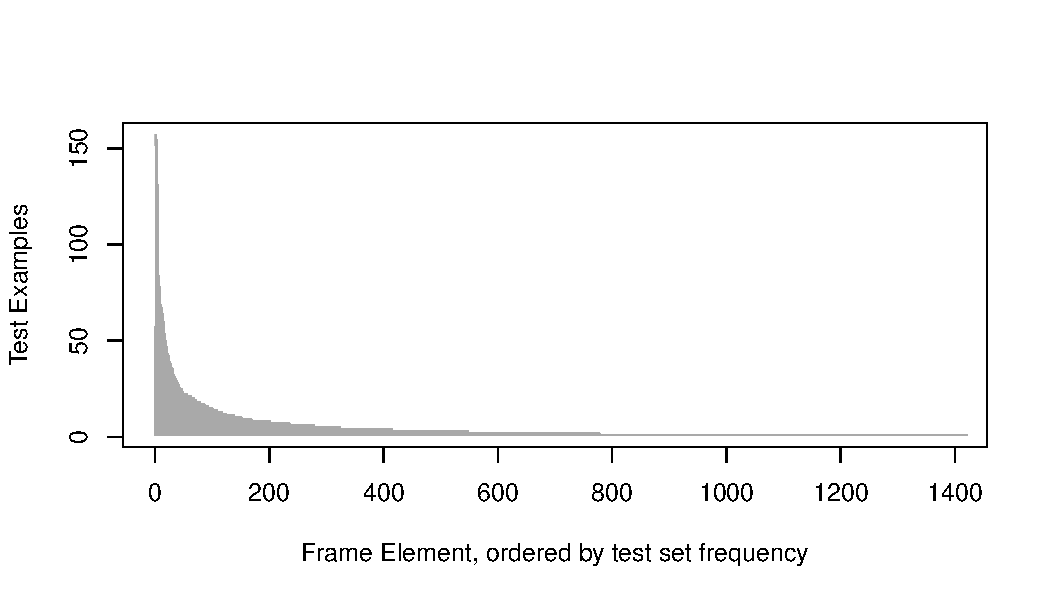
\includegraphics[width=\textwidth]{fig/num_instances}
%		\caption{Frequency of each role appearing in the test set.}\label{fig:num_inst}
%	\end{subfigure}
%	\begin{subfigure}[b]{0.5\textwidth}
%		\vspace{-1cm}
		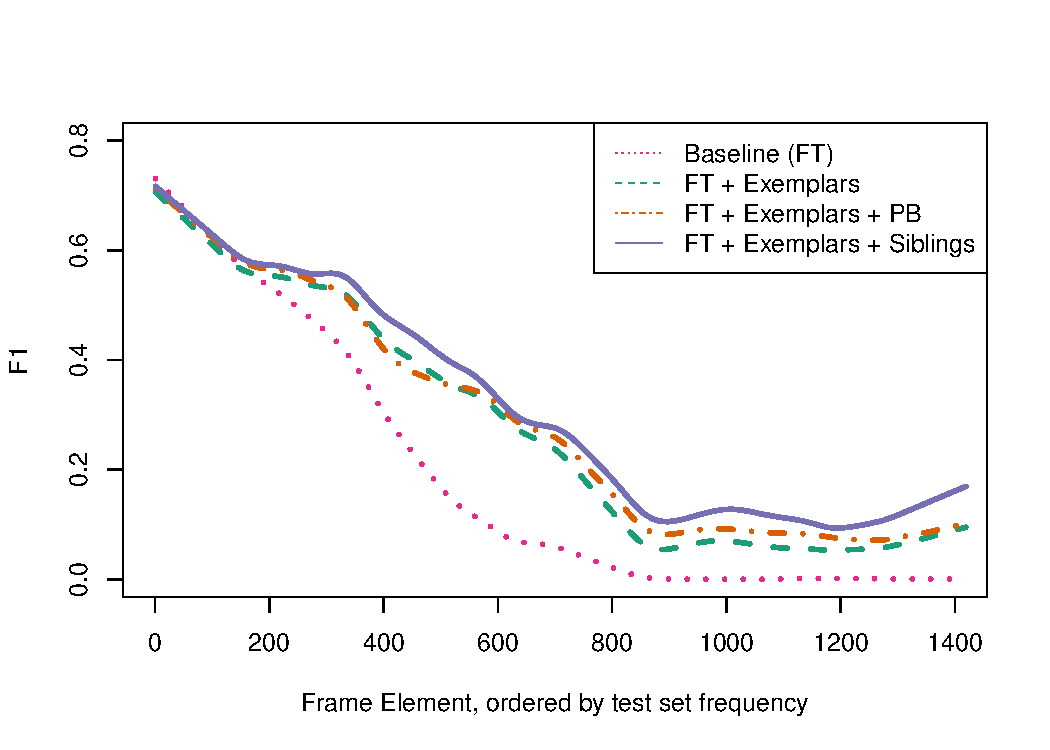
\includegraphics[width=0.5\textwidth]{fig/f1_sorted_by_num_instances}
%		\caption{$F_1$ of the best methods compared with the baseline.}\label{fig:coolplot}
%	\end{subfigure}
%	\caption{Count and $F_1$ for each role appearing in the test
%	set. $F_1$ values have been smoothed with \texttt{loess}, with
%	a smoothing parameter of 0.2.}
\caption{\label{fig:coolplot}$F_1$ by role, ranked by frequency
  (smoothed using \texttt{loess} with parameter 0.2). \nascomment{make
  font bigger in the figure, and make lines thicker}}
\end{figure}


% \paragraph{Combining all resources.}
The last two rows of 
\cref{tbl:results} show the performance upon combining the best
approaches.  Both models use full-text and exemplars for training; the
first uses PropBank as guide features, and the second adds hierarchy (sibling) features.  
The best result is the former, gaining 3.95\% $F_1$ over the baseline.
\paragraph{Full-system.} When using the frame output of \cite{hermann-14}, $F_1$
improves by 1.1, from 66.78 for the baseline, to 67.91 for our combined
model (last row in \cref{tbl:results}).
\mk{New text above and below.. please check. Do we want to quote the result: 70.27 on full-system 
from Tackstrom 2015? If you see the plot I sent over email, they
are doing much better than SEMAFOR on the frequent roles. We improve F1 on the rare ones.
Hence should we say that if we use their system as baseline, we would still
expect to see benefits from the additional resources? }
\st{this isn't actually the baseline SEMAFOR system, is it? I thought it was
using Hermann frames, which is not part of SEMAFOR.}


% Here, both models use the optimal training data configuration: (FT+exemplars) but differ in the feature augmentation used. 
% We find that the model that uses the hierarchy achieves the best recall, and the PB-SRL guide features result in the 
% best precision. %This result is intuitive because we expect the hierarchy to help \mk{insert good explanation here}.
% Our best result of 63.07 beats the baseline by 3.95 F points.
\paragraph{Role-level evaluation.}
\Cref{fig:coolplot} shows $F_1$ per frame element, for the
baseline and the two best models from \cref{tbl:results}.  Each
$x$-axis value is one role, sorted by decreasing frequency (the
distribution, not shown for space, is Zipf-like).  For frequent roles,
performance is similar; our models achieve gains on rarer roles.

\paragraph{Additional results.} Experiments with another resource,
SemLink \citep{bonial-13}, yielded negative results. We also evaluated
all models on a test set sampled from the exemplars, which differs in distribution from the FT data.
These results are provided in the supplement.

\finalversion{\nss{impact of automatic frames?}}
%\subsection{Frame element--level evaluation}
%The results so far have discussed the overall improvement in $F_1$, but do not present a detailed picture of how we gain from the additional
%coverage. Towards this, we present a frame-element i.e role type level analysis comparing the best results with the baseline.


%\section{Related Work}


% \citet{tackstrom-15} is the most recent work on frame-semantic argument identification.
% They present an efficient dynamic program for solving the joint role assignment problem (equation~\ref{eq:args}), and show that using it at training time is helpful.
% Their work is complementary to our own.

% \nss{Dipanjan's other papers (focusing on different parts of the task)}


%\nss{multitask learning?}
%\mk{there's no room for citing MTL.. we can do that later}

\section{Conclusion}

We have empirically shown that auxiliary semantic resources
can benefit the challenging task of frame-semantic role labeling. 
The significant gains come from the FrameNet exemplars and the FrameNet hierarchy, with
some signs that data annotated with the PropBank scheme can be leveraged as well.
\nss{release of code and models}

%\mk{For short version: the rest of the conclusion is already present in the Results section}
%Complementary gains on the standard full-text evaluation are achieved
%by including the FrameNet exemplars in the training data 
%and by grouping features according to the FrameNet hierarchy. 
%There are smaller, but nevertheless promising, signs that data annotated 
%with the PropBank scheme can be leveraged as well.
%In addition to making SRL more \emph{accurate}, a parallel evaluation on a sample of exemplars suggests the 
%improved models are also more \emph{robust}, capturing a broader swath of the English language.

\finalversion{We are optimistic that future improvements to lexical semantic resources, 
including planned changes for PropBank \citep{bonial-14} and SemLink \citep{bonial-13}, 
will lead to further gains in this task. 
Moreover, the techniques discussed here could be further explored 
using semi-automatic mappings between lexical resources \citep[such as UBY;][]{gurevych-12}, 
and correspondingly, this task could be used to extrinsically validate those mappings.}
\finalversion{\nss{release of code and models}}

\finalversion{\section*{Acknowledgments}

FUNDING}

\smaller

\bibliographystyle{style/aclnat}
% you bib file should really go here
\setlength{\bibsep}{1pt}
{\fontsize{10}{12.25}\selectfont
\bibliography{argid}}


\end{document}
